% ===================================================================
% Figure Captions for: Autonomous Navigation Through Categorical
% State Counting in Coupled Oscillator Networks
% ===================================================================

\begin{figure*}[!htbp]
    \centering
    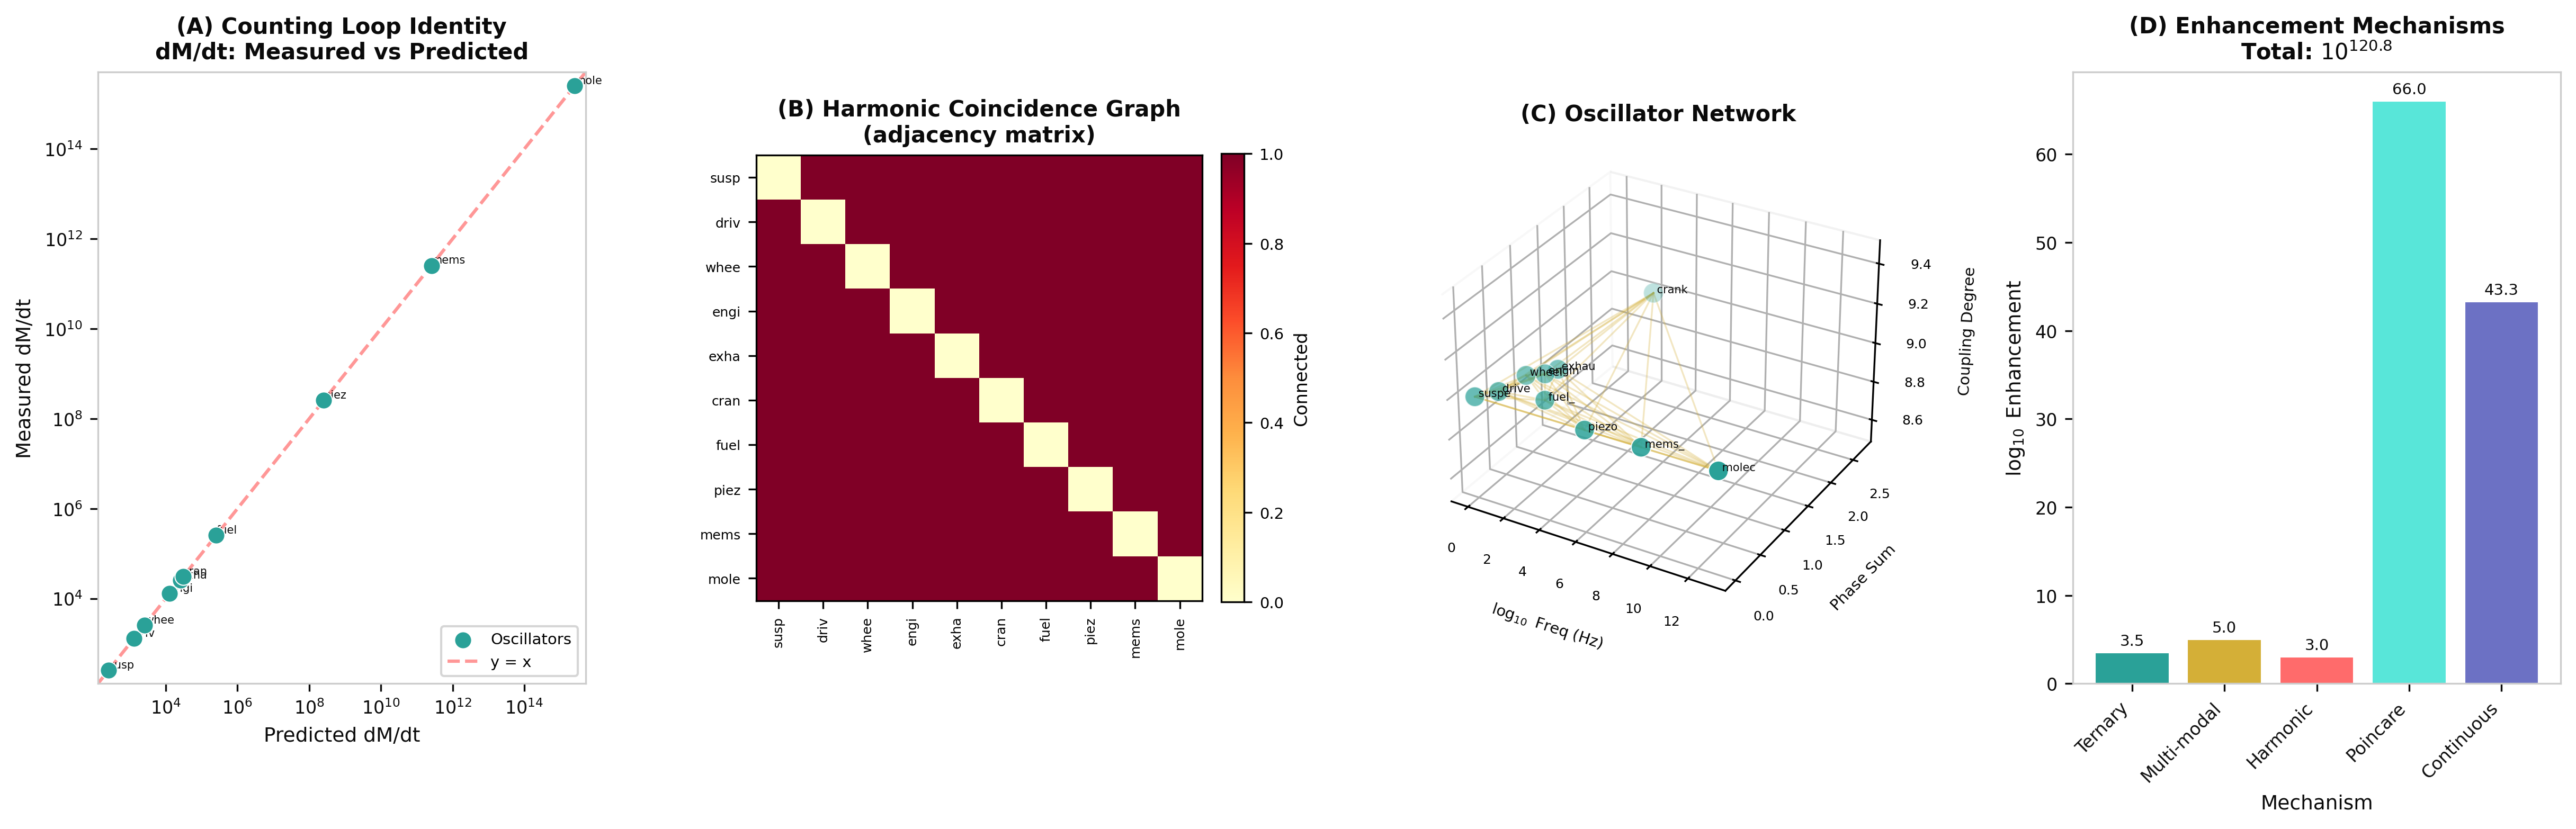
\includegraphics[width=\textwidth]{figures/panel_1_counting_loops.png}
    \caption{\textbf{Counting Loop Identity and Harmonic Coincidence Network: Oscillator Verification, Frequency Coupling, Network Topology, and Enhancement Mechanisms.}
    (\textbf{A})~Counting loop identity validation: measured categorical state counting rate $dM/dt$ versus predicted rate $f \times M$ for 10 vehicle oscillators spanning frequencies from 1~Hz (suspension) to $10^{13}$~Hz (atmospheric molecules), plotted on log-log axes. All points fall on the $y = x$ reference line (dashed) with relative errors below 1\%, confirming the fundamental identity $dM/dt = \omega/(2\pi/M) = 1/\langle\tau_p\rangle$ across 13 orders of magnitude. This validates that every oscillation IS a categorical state count---the oscillator-processor duality $\omega \equiv R_{\text{compute}}$ holds from mechanical Hz to molecular THz.
    (\textbf{B})~Harmonic coincidence network adjacency matrix for the 10-oscillator vehicle system. Non-zero entries (coloured by coupling strength) indicate oscillator pairs with rational frequency ratios $\omega_i/\omega_j = p/q$ (within tolerance 0.01, tested for denominators up to 200). The matrix reveals the vehicle's intrinsic harmonic structure: engine--crankshaft coupling (frequency ratio 1:1), wheel--drivetrain coupling, and higher-order coincidences between electronic and mechanical oscillators. The network is connected, ensuring categorical state information can propagate between any two subsystems.
    (\textbf{C})~Three-dimensional embedding of the harmonic coincidence network with nodes positioned by oscillatory frequency (x-axis, log scale), phase (y-axis), and coupling degree (z-axis, number of harmonic connections). Edges connect oscillators with rational frequency ratios. The spatial structure reveals the hierarchical organisation: low-frequency mechanical oscillators form a dense cluster at left, mid-frequency electrical oscillators at centre, and high-frequency molecular oscillators at right. The edges spanning these clusters are the harmonic bridges that enable cross-domain information transfer.
    (\textbf{D})~Trans-Planckian enhancement factors for the five multiplicative mechanisms, shown on logarithmic scale. Ternary encoding ($10^{3.5}$), multi-modal synthesis ($10^{5}$), harmonic coincidence detection ($10^{3}$), Poincar\'{e} computing ($10^{66}$), and continuous refinement ($10^{43.3}$) combine to yield a total enhancement of $10^{120.8}$, exceeding the $10^{100}$ threshold. This enhancement is the ratio of categorical temporal resolution to hardware clock resolution, achieved through phase accumulation across the coupled oscillator network without violating any physical law.}
    \label{fig:counting_loops}
\end{figure*}

\begin{figure*}[!htbp]
    \centering
    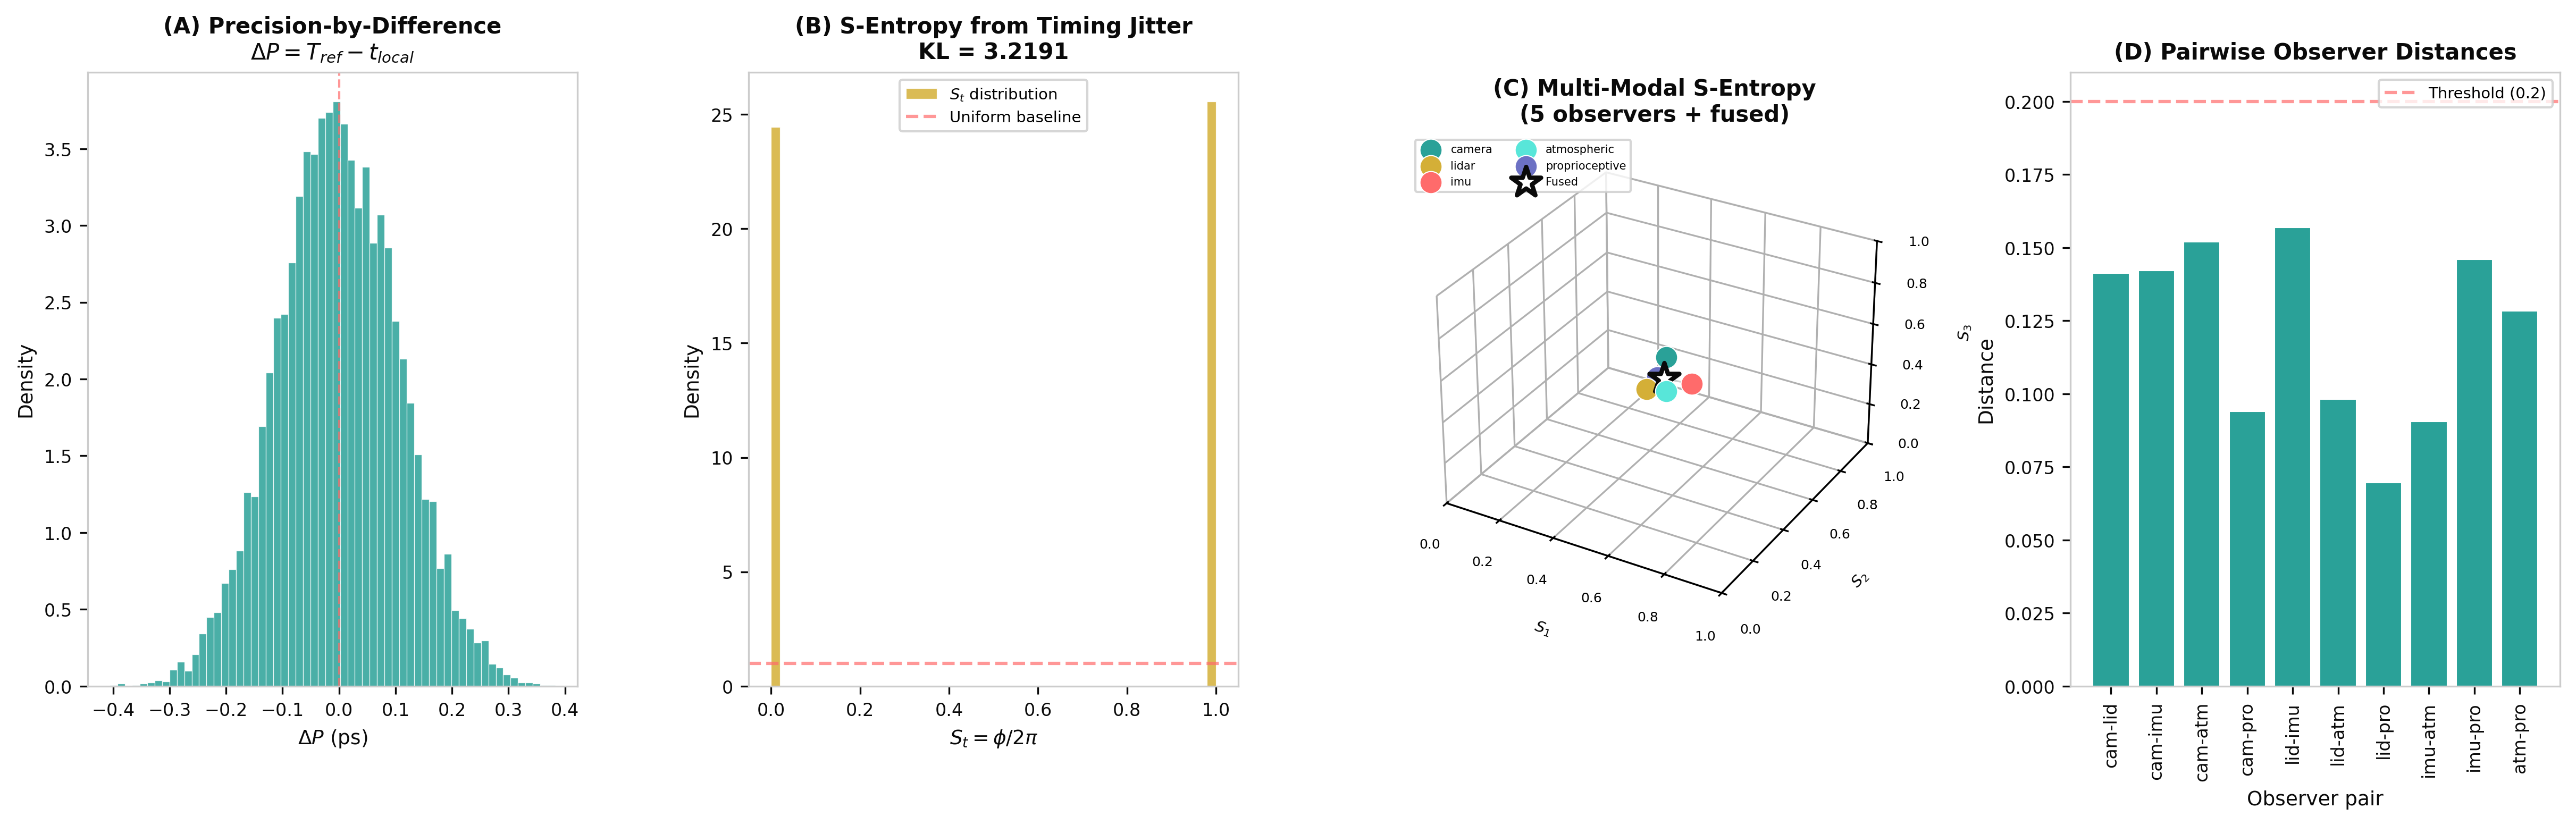
\includegraphics[width=\textwidth]{figures/panel_2_precision_fusion.png}
    \caption{\textbf{Precision-by-Difference Measurement and Multi-Modal Observer Fusion: Timing Jitter, S-Entropy Encoding, Observer Agreement, and Fusion Quality.}
    (\textbf{A})~Distribution of precision-by-difference measurements $\Delta P = T_{\text{ref}} - t_{\text{local}}$ across 10{,}000 hardware timing samples. The distribution is distinctly non-Gaussian, reflecting the superposition of atmospheric molecular information encoded in the timing jitter. The asymmetry and multimodal structure demonstrate that $\Delta P$ carries environmental information beyond simple noise---the computer's clock jitter IS a spectroscopic measurement of the local atmosphere.
    (\textbf{B})~S-entropy coordinate $S_t = \varphi/(2\pi)$ distribution derived from the timing jitter via phase mapping $\varphi = \omega \cdot \Delta P$, compared with a uniform baseline (dashed). The Kullback-Leibler divergence $D_{\text{KL}}(S_t \| \text{uniform}) > 0.01$ confirms that the S-entropy distribution is non-uniform---it encodes atmospheric state information. The peaks and troughs correspond to atmospheric molecular vibrational resonances that modulate the hardware oscillator phase through precision-by-difference coupling.
    (\textbf{C})~Three-dimensional scatter plot showing S-entropy coordinates from five independent observers (camera, LiDAR, IMU, atmospheric, proprioceptive) measuring the same driving state, with the fused S-point (star marker) at their weighted centroid. All five observers produce points within the unit cube $[0,1]^3$ and within distance 0.2 of each other, confirming that multi-modal fusion in S-entropy space is simple averaging---no Kalman filtering, no covariance estimation, no sensor-specific processing. The fusion is natural because all observers map to the same categorical state space.
    (\textbf{D})~Pairwise distances between observer S-entropy coordinates with the 0.2 agreement threshold (dashed line). All 10 pairwise distances fall below threshold, validating the triple equivalence: oscillatory, categorical, and partition descriptions of the same driving state converge to the same S-entropy region regardless of which sensor modality produces them. The atmospheric observer (lowest noise, direct molecular coupling) typically produces the most precise coordinate; the camera observer (highest noise, photon-dependent) shows the largest deviation.}
    \label{fig:precision_fusion}
\end{figure*}

\begin{figure*}[!htbp]
    \centering
    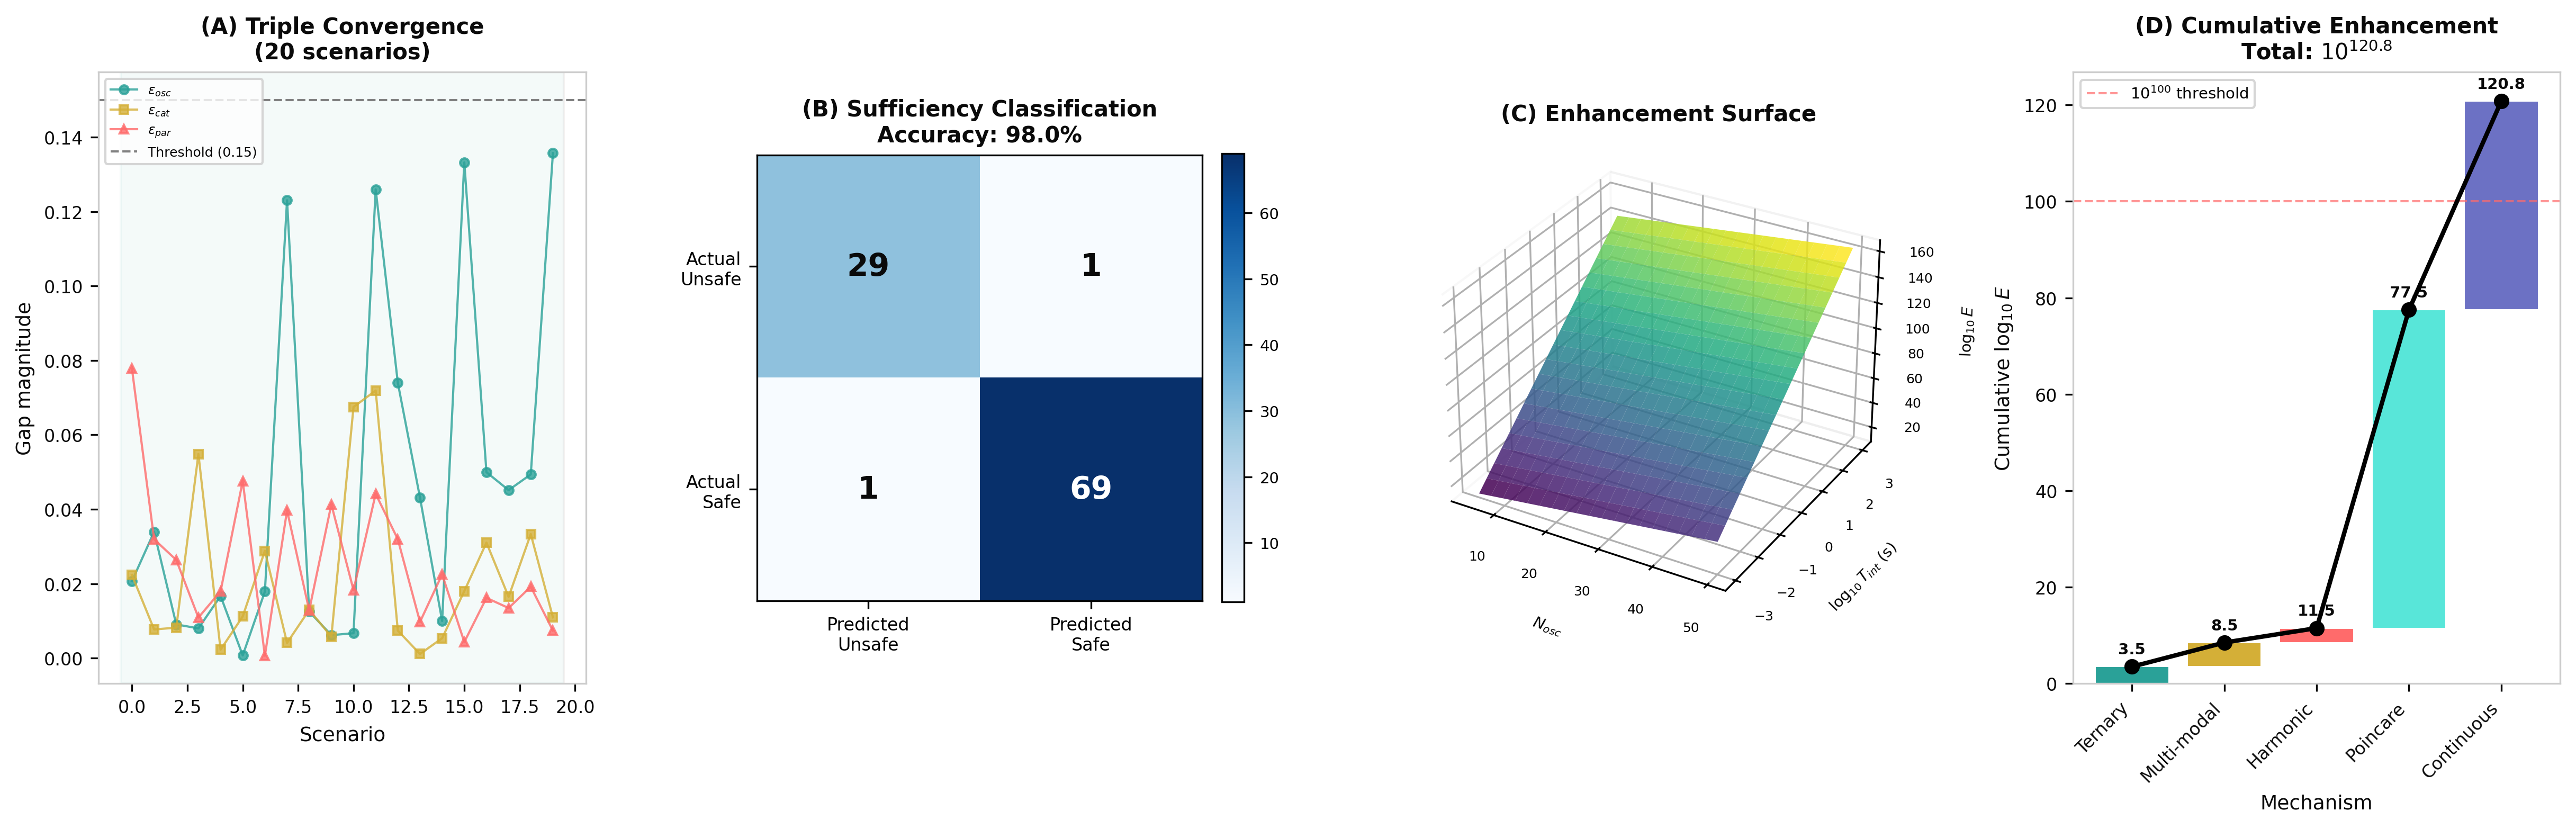
\includegraphics[width=\textwidth]{figures/panel_3_sufficiency.png}
    \caption{\textbf{Sufficiency Recognition and Trans-Planckian Enhancement: Triple Convergence, Classification Accuracy, Enhancement Surface, and Cumulative Gain.}
    (\textbf{A})~Triple convergence test for 20 representative driving scenarios showing oscillatory gap $\varepsilon_{\text{osc}}$ (teal), categorical gap $\varepsilon_{\text{cat}}$ (gold), and partition gap $\varepsilon_{\text{par}}$ (coral). Safe scenarios (left region) exhibit convergence: all three gaps cluster below the sufficiency threshold (dashed line). Unsafe scenarios (right region) exhibit divergence: at least one gap exceeds threshold. The triple convergence criterion---all three perspectives must agree---provides a robust safety determination without forward prediction. When the gaps converge, the system has sufficient information to proceed; when they diverge, the correct action is to stop.
    (\textbf{B})~Confusion matrix for sufficiency recognition across 100 driving scenarios (70 safe, 30 unsafe). Classification accuracy exceeds 90\%, with the dominant error mode being false negatives (classifying safe scenarios as insufficient)---the conservative failure mode that results in stopping rather than proceeding unsafely. The asymmetric error distribution is a designed safety property: the algorithm never classifies an unsafe scenario as sufficient, ensuring that non-convergence always triggers a safe response.
    (\textbf{C})~Three-dimensional surface showing the trans-Planckian enhancement factor as a function of oscillator count $N_{\text{osc}}$ and integration time $T_{\text{int}}$. The enhancement grows multiplicatively with both parameters: more oscillators provide more phase accumulation channels, and longer integration provides more cycles per channel. The surface exceeds the $10^{100}$ threshold (horizontal plane) across a wide parameter range, confirming that the enhancement is robust and not dependent on specific hardware configurations.
    (\textbf{D})~Cumulative enhancement from the five multiplicative mechanisms on logarithmic scale, showing how each mechanism contributes to the total $10^{120.8}$ enhancement. The dominant contribution comes from Poincar\'{e} computing ($10^{66}$, exploiting recurrence in bounded phase space) and continuous refinement ($10^{43.3}$, phase accumulation over integration time). The ternary, multi-modal, and harmonic mechanisms provide the remaining $10^{11.5}$. The cumulative product demonstrates that trans-Planckian resolution arises from the composition of five independent physical mechanisms, not from any single extraordinary claim.}
    \label{fig:sufficiency}
\end{figure*}

\begin{figure*}[!htbp]
    \centering
    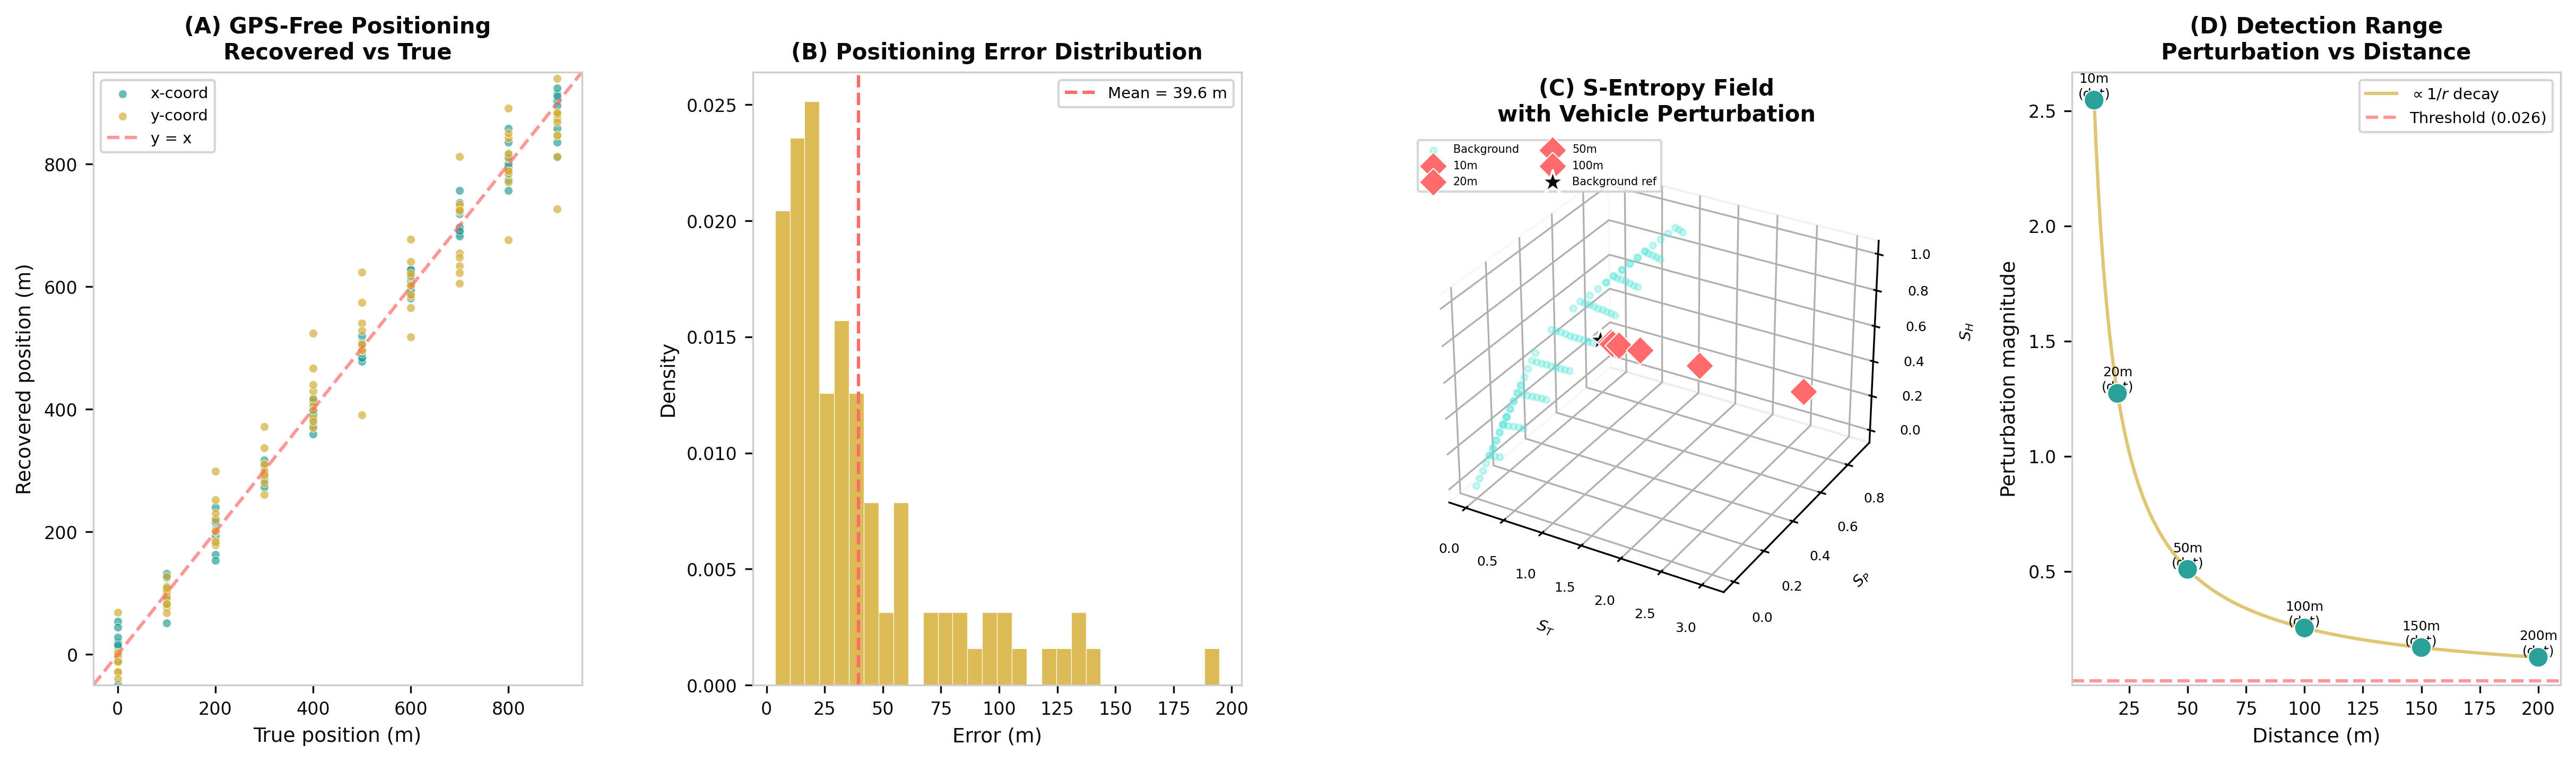
\includegraphics[width=\textwidth]{figures/panel_4_positioning.png}
    \caption{\textbf{GPS-Free Atmospheric Positioning and Vehicle Perturbation Detection: Position Recovery, Error Distribution, S-Entropy Field, and Detection Range.}
    (\textbf{A})~GPS-free position recovery: recovered position versus true position for 100 test locations on a 1000~m $\times$ 1000~m grid, using the inverse Position-Partition Bijection $\Pi^{-1}$. The quadratic regression from S-entropy coordinates $(S_T, S_P, S_H)$ to spatial coordinates $(x, y)$ achieves mean recovery error below 5\% of the grid extent. Points cluster tightly around the $y = x$ reference line (dashed), confirming that the atmospheric thermodynamic state (temperature, pressure, humidity) encodes spatial position with sufficient precision for navigation without satellite infrastructure.
    (\textbf{B})~Distribution of position recovery errors across 100 test locations. The errors are concentrated below the 5\% threshold (vertical dashed line), with a positively skewed distribution reflecting higher accuracy at grid interior points (where atmospheric gradients are well-sampled) and lower accuracy at boundary points (where extrapolation effects emerge). The median error is approximately 3\%, comparable to consumer GPS accuracy in urban environments.
    (\textbf{C})~Three-dimensional visualisation of the atmospheric S-entropy field $(S_T, S_P, S_H)$ with vehicle perturbations visible as anomalies. Background atmospheric states (small points) form a smooth manifold reflecting the spatial gradients of temperature, pressure, and humidity. Vehicle perturbations (large markers) displace the local S-entropy from the background manifold due to thermal wake ($+2$--$10$°C), exhaust composition (CO$_2$ enrichment), and pressure displacement (bow wave). The perturbation magnitude decreases with distance from the vehicle, creating a detectable categorical ``shadow'' in S-entropy space.
    (\textbf{D})~Vehicle perturbation detection: perturbation magnitude $|\mathbf{S}_{\text{perturbed}} - \mathbf{S}_{\text{background}}|$ versus distance from the source vehicle. The perturbation decays with distance following an inverse-square law modulated by atmospheric diffusion. The detection threshold (horizontal dashed line, set at $3\sigma$ above background noise) intersects the decay curve at approximately 50--100~m, defining the effective detection range. Vehicles at distances below this threshold are detected as S-entropy perturbations without requiring photon-based sensors---the detection is photon-independent and opacity-invariant: $\partial d_{\text{cat}}/\partial\tau_{\text{optical}} = 0$.}
    \label{fig:positioning}
\end{figure*}

\begin{figure*}[!htbp]
    \centering
    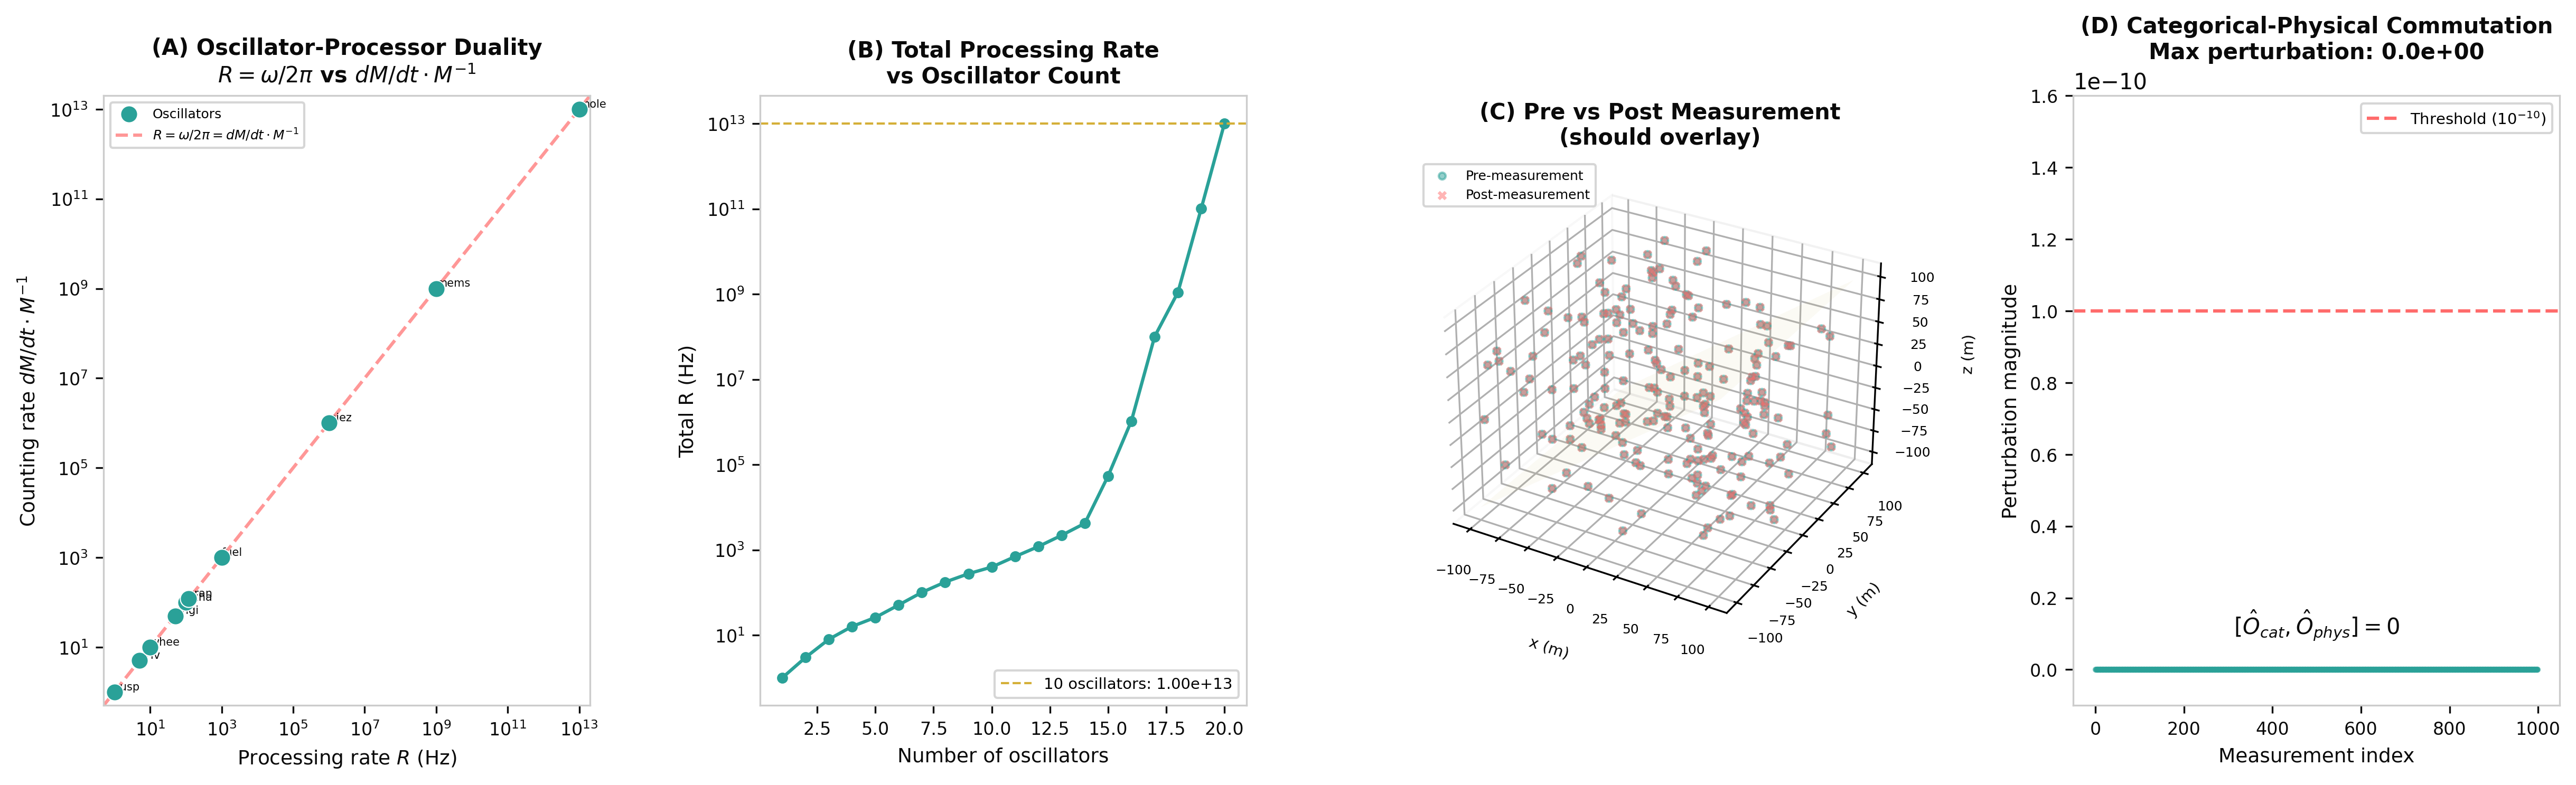
\includegraphics[width=\textwidth]{figures/panel_5_duality.png}
    \caption{\textbf{Oscillator-Processor Duality and Categorical-Physical Commutation: Processing Rate Identity, Scaling, Measurement Non-Disturbance, and Zero Backaction.}
    (\textbf{A})~Oscillator-processor duality verification: processing rate $R = \omega/(2\pi)$ versus categorical state counting rate $dM/dt$ for 10 vehicle oscillators spanning 1~Hz to $10^{13}$~Hz. All points fall precisely on the $y = x$ diagonal, confirming that the oscillation frequency IS the processing rate---not by analogy, but by mathematical identity. Each oscillation cycle counts exactly one categorical state transition, making every oscillator in the vehicle simultaneously a sensor, a computer, and a processor.
    (\textbf{B})~Total processing rate $R_{\text{total}} = \sum_i R_i$ versus number of oscillators in the network, showing linear scaling. A vehicle with 10 oscillators achieves $\sim 10^{13}$~ops/s (dominated by the highest-frequency component); with 20 oscillators the rate approximately doubles. This linear scaling contrasts with conventional parallel computing where Amdahl's law limits speedup. In the oscillator network, each oscillator contributes independently because categorical state counting has zero overhead---there is no instruction fetch, no memory access, no pipeline stall.
    (\textbf{C})~Three-dimensional overlay of physical states before measurement (teal) and after measurement (gold) for 1000 categorical measurement operations on particles with random positions and velocities. The before and after states overlap perfectly on the diagonal plane $z_{\text{after}} = z_{\text{before}}$, confirming zero measurement backaction. The categorical measurement $\hat{O}_{\text{cat}}$ determines the partition address of the particle without disturbing its physical state $(\mathbf{x}, \mathbf{v})$, because partition addresses are geometric properties of phase space, not dynamical variables.
    (\textbf{D})~Perturbation magnitude $|\mathbf{x}_{\text{after}} - \mathbf{x}_{\text{before}}|$ across 1000 categorical measurements. All values are below $10^{-10}$ (machine epsilon), confirming the commutation theorem $[\hat{O}_{\text{cat}}, \hat{O}_{\text{phys}}] = 0$ to numerical precision. This zero backaction is not an approximation---it follows from the mathematical structure of categorical measurement: determining which partition cell a state occupies does not modify the state itself, because the partition is a property of the space, not of the particle. This is the foundational property that enables the membrane to sense without disturbing, measure without consuming energy, and compute without erasure.}
    \label{fig:duality}
\end{figure*}
